In each of the following exercises, find the equation of the circle with the following parameters
\begin{enumerate}[label=\thesection.\arabic*,ref=\thesection.\theenumi]
\numberwithin{equation}{enumi}
\numberwithin{figure}{enumi}
\numberwithin{table}{enumi}
 \item centre $(0,2)$ and radius $2$
	 \\
		\solution
\label{chapters/11/11/1/1}
\\
\iffalse
\documentclass[12pt]{article}
\usepackage{graphicx}
\usepackage{amsmath}
\usepackage{mathtools}
\usepackage{gensymb}

\newcommand{\mydet}[1]{\ensuremath{\begin{vmatrix}#1\end{vmatrix}}}
\providecommand{\brak}[1]{\ensuremath{\left(#1\right)}}
\providecommand{\norm}[1]{\left\lVert#1\right\rVert}
\newcommand{\solution}{\noindent \textbf{Solution: }}
\newcommand{\myvec}[1]{\ensuremath{\begin{pmatrix}#1\end{pmatrix}}}
\let\vec\mathbf

\begin{document}
\begin{center}
\textbf\large{CHAPTER-11 \\ CIRCLES}

\end{center}
\section*{Excercise 11.1}

Q1.Find the equation of the circle with centre $(0,2)$ and radius 2.

\solution
\fi
The equation of the circle is given by 
\begin{align}
	\norm{\vec{x}}^{2} + 2\vec{u}^{\top}\vec{x} + f = 0
\end{align}
From the given information,
\begin{align}
	\vec{c} = \myvec{0\\2} \text{ and } r = 2,
\end{align}
Since 
\begin{align}
	\vec{u} = -\vec{c} \text{ and } f = \norm{\vec{u}}^{2} - r^{2},
\end{align}
substituting numerical values, 
\begin{align}
	\vec{u} = \myvec{0\\-2},
	f 
	  = 0
\end{align}
Thus, the equation of circle is obtained as
\begin{align}
	\norm{\vec{x}}^2 + 2\myvec{0 & 2}\vec{x} = 0
\end{align}
See Fig. \ref{fig:11/11/1/1/Fig1}	
\begin{figure}[!h]
	\begin{center} 
	    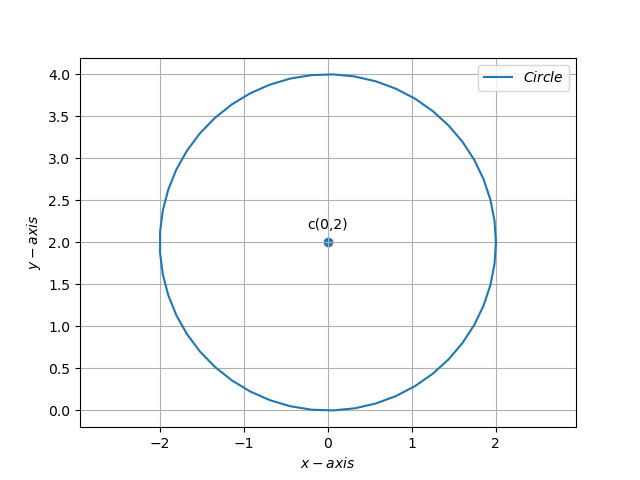
\includegraphics[width=\columnwidth]{chapters/11/11/1/1/figs/circ1}
	\end{center}
\caption{}
\label{fig:11/11/1/1/Fig1}
\end{figure}



  \item centre $(-2,3)$ and radius 4

  \item centre $\left(\frac{1}{2}, \frac{1}{4}\right)$ and radius $\frac{1}{12}$

  \item centre $(1,1)$ and radius $\sqrt{2}$

  \item centre $(-a,-b)$ and radius $\sqrt{a^{2}-b^{2}}$.
\end{enumerate}


In each of the following exercises,  find the centre and radius of the circles.
\begin{enumerate}[resume*]
\item  $(x+5)^{2}+(y-3)^{2}=36$ 
\item  $x^{2}+y^{2}-4 x-8 y-45=0$
\item  $x^{2}+y^{2}-8 x+10 y-12=0$ 
\item  $2 x^{2}+2 y^{2}-x=0$
\end{enumerate}

\begin{enumerate}[resume*]
  \item Find the equation of the circle passing through the points $(4,1)$ and $(6,5)$ and whose centre is on the line $ 4x+y=16. $

  \item Find the equation of the circle passing through the points $(2,3)$ and $(-1,1)$ and whose centre is on the line $x-3y-11=0$.
\label{chapters/11/11/1/11}
\\
\iffalse
\documentclass[journal,10pt,twocolumn]{article}
\usepackage{graphicx}
\usepackage[margin=0.5in]{geometry}
\usepackage[cmex10]{amsmath}
\usepackage{array}
\usepackage{booktabs}
\usepackage{mathtools}
\usepackage{multicol}
\usepackage[utf8]{inputenc}
\title{\textbf{Conic section Assignment}}
\author{Thoutu Rahul Raj}
\date{October 2022}


\providecommand{\norm}[1]{\left\lVert#1\right\rVert}
\providecommand{\abs}[1]{\left\vert#1\right\vert}
\let\vec\mathbf
\newcommand{\myvec}[1]{\ensuremath{\myvec{#1}}}
\newcommand{\mydet}[1]{\ensuremath{\begin{vmatrix}#1\end{vmatrix}}}
\providecommand{\brak}[1]{\ensuremath{\left(#1\right)}}
\providecommand{\lbrak}[1]{\ensuremath{\left(#1\right.}}
\providecommand{\rbrak}[1]{\ensuremath{\left.#1\right)}}
\providecommand{\sbrak}[1]{\ensuremath{{}\left[#1\right]}}

\begin{document}
\maketitle
\section{Problem Statement}
Find the equation of the circle passing through the points (2,3) and (-1,1) and whose centre is on the line $x-3y-11=0$
\fi
\solution See Fig. 
	\begin{figure}[!ht]
		\centering
 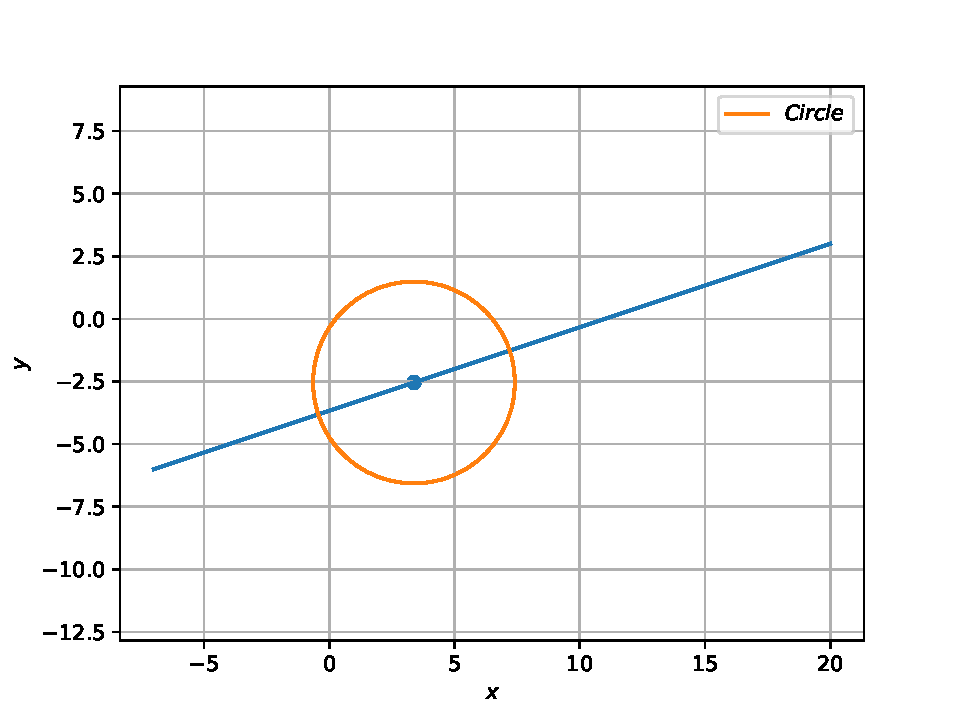
\includegraphics[width=\columnwidth]{chapters/11/11/1/11/figs/fig.pdf}
		\caption{}
		\label{fig:11/11/1/11}
  	\end{figure}
\iffalse
}
\section{Solution}
To Find : The equation of circle.
Given , points passing through circle (2,3) and (-1,1), And equation of line passing through the center of circle x-3y-11=0
\begin{align}
    \vec{x}^{\top}\vec{V}\vec{x}+2\vec{u}^{\top}\vec{x}+f=0\\
	\vec{V} &= \myvec{1 & 0\\0 & 1},
	\\
	\vec{u} &= \myvec{h\\k},
	\\
	f &= f
\end{align}


which is the equation of a circle. 
And h,k,C are unknown values we should find
\fi
From 
	\eqref{eq:circ-eq}, and the given information, 
\begin{align}
	\norm{\vec{P}}^2 + 2 \vec{u}^{\top}\vec{P} + f &= 0
	\\
	\norm{\vec{Q}}^2 + 2 \vec{u}^{\top}\vec{Q} + f &= 0
	\\
	-\vec{n}^{\top}\vec{u} &=c
\end{align}
by noting that the centre of the circle is $-\vec{u}$.
Substituting numerical values, we obtain the matrix equation
\begin{align}
	\label{eq:vertex_system}
	\myvec{4&6&1\\-2& 2&1\\-1& 3&0}\myvec{\vec{u}\\f} = \myvec{-13\\-2 \\11}\\
\end{align}
The augmented matrix for \eqref{eq:vertex_system} can be expressed as
\begin{align}
	\xleftrightarrow[]{1/4 R_1 \leftrightarrow R_1}\myvec{1&3/2&.1/4&\vrule&-13/4\\-2&2&1&\vrule&-2\\-1&3&0&\vrule&11}
\end{align}
which can be reduced to echelon form using row operations to obtain 
\iffalse
\begin{align}
		\xleftrightarrow[]{-1/2R_2 \leftrightarrow R_2}
		\myvec{1&3/2&1/4&\vrule&-13/4\\1&-1&-1/2&\vrule&1\\-1&3&0&\vrule&11}\\
	     \xleftrightarrow[]{-1R_3 \leftrightarrow R_3}	
\myvec{1&3/2&1/4&\vrule&-13/4\\1&-1&-1/2&\vrule&1\\1&-3&0&\vrule&-11}\\
		\xleftrightarrow[]{R_2-1.R_1 \leftrightarrow R_2}
		\myvec{1&3/2&1/4&\vrule&-13/4\\0&-5/2&-3/4&\vrule&17\\1&-3&0&\vrule&-11}\\
	     \xleftrightarrow[]{R_3-1.R_1 \leftrightarrow R_3}
	     \myvec{1&3/2&1/4&\vrule&-13/4\\0&-5/2&-3/4&\vrule&17/4\\0&9/2&-1/4&\vrule&-31/4}\\
	     \xleftrightarrow[]{-2/5R_2 \leftrightarrow R_2}
	  \myvec{1&3/2&1/4&\vrule&-13/4\\0&1&3/10&\vrule&17/10\\0&9/2&-1/4&\vrule&-31/4}
\end{align}
\begin{align}
	      \xleftrightarrow[]{-2/9R_3 \leftrightarrow R_3}	
\myvec{1&3/2&1/4&\vrule&-13/4\\1&-1&-1/2&\vrule&1\\1&-3&0&\vrule&-11}\\
		\xleftrightarrow[]{R_3-1.R_2 \leftrightarrow R_3}
\myvec{1&3/2&1/4&\vrule&-13/4\\0&1&3/10&\vrule&-17/10\\0&0&-11/45&\vrule&154/45}\\		
	     \xleftrightarrow[]{-45/11R_3 \leftrightarrow R_3}
	     \myvec{1&3/2&1/4&\vrule&-13/4\\0&1&3/10&\vrule&-17/10\\0&0&1&\vrule&-14}\\
	     \xleftrightarrow[]{R_2-3/10R_3 \leftrightarrow R_2}
	     \myvec{1&3/2&1/4&\vrule&-13/4\\0&1&0&\vrule&5/2\\0&0&1&\vrule&-14}\\	
	      \xleftrightarrow[]{R_1-1/4R_3 \leftrightarrow R_1}
	      	     \myvec{1&3/2&0&\vrule&1/4\\0&1&0&\vrule&5/2\\0&0&1&\vrule&-14}\\
	       \xleftrightarrow[]{R_1-3/2R_2 \leftrightarrow R_1}	
\myvec{1&0&0&\vrule&-7/2\\0&1&0&\vrule&5/2\\0&0&1&\vrule&-14}\\
\end{align}
yielding 
\fi
\begin{align}
\vec{u}=\myvec{-7/2 \\5/2 },
f=-14
\end{align}
\iffalse
\end{align}
from u and f we can find radius
\begin{align}
 r = \sqrt{\norm{\vec{(u)}}^2-f} 
\end{align}
\begin{align}
r = \sqrt{65/4}
\end{align}
And, from them we can find the equation of circle.\\
 \begin{align}
\vec{x}^{\top}\vec{V}\vec{x}+2\vec{u}^{\top}\vec{x}+f=0
\end{align}	
$\vec{V}$ = $\myvec{
 1 & 0\\
 0 & 1
 }$, 
  $\vec{u}$=$\vec{\myvec{7/2 \\-5/2 }}$
  f = 14
steps for constructing above figure are:  
\begin{center}
\begin{tabular}{|c|c|c|}
	\hline
	\textbf{Symbol}&\textbf{Value}&\textbf{Description}\\
	\hline
	$r$&$\sqrt{65/4}$&Radius of the circle\\
	\hline
	\textbf{C}&$\
	\myvec{
		7/2 \\
		-5/2 \\
	}$
	&center of circle\\
	\hline
\end{tabular}
\end{center}
\vspace{1mm}

\section{ Construction}
%\includegraphics[scale=0.5]{../Documents/co.pdf} 
%\includegraphics[scale=0.5]{co.pdf} 
%\vspace{3mm}
%\url{https://github.com/9705701645/FWC/blob/main/co.py}
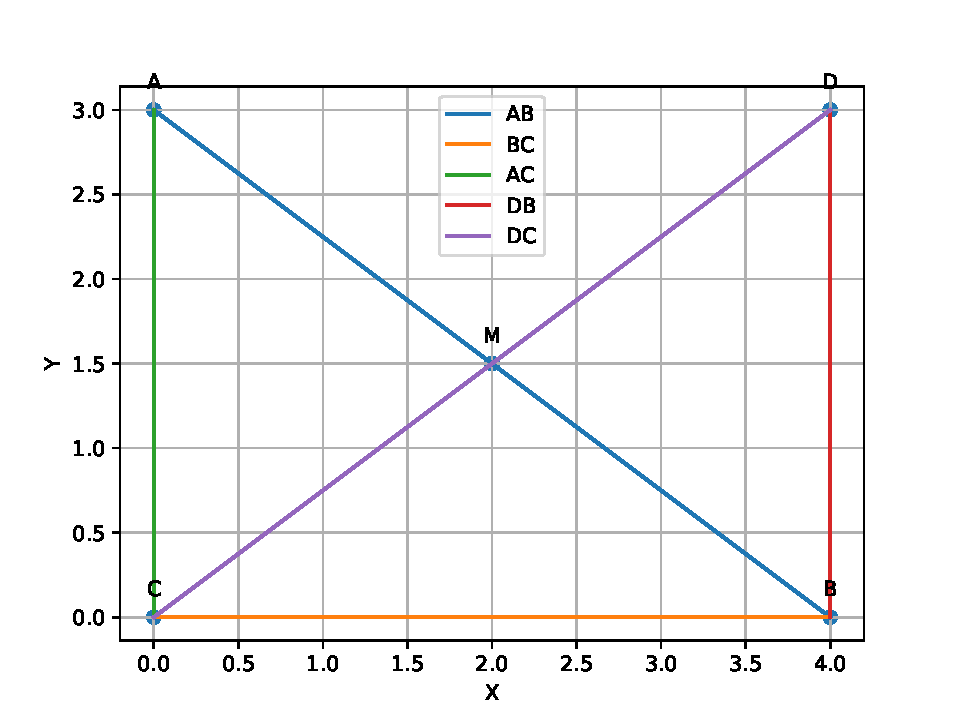
\includegraphics[scale=1]{fig.pdf} 
%\begin{multicols}
 %Download the code \\
%\href{https://github.com/9705701645/FWC/blob/main/co.py}{Assignment-5}.
%\end{multicols}
\end{document}


\fi

  \item Find the equation of the circle with radius 5 whose centre lies on $x$-axis and passes through the point $(2,3)$.
\label{chapters/11/11/1/12}
\\
\iffalse
\documentclass[a4paper,12pt,twocolumn]{article}
\usepackage{graphicx}
\usepackage[margin=0.5in]{geometry}
\usepackage[cmex10]{amsmath}
\usepackage{array}
\usepackage{gensymb}
\usepackage{booktabs}
\title{Conic Assignment}

\author{Ravi Sumanth Muppana- FWC22003}
\date{September 2022}
\providecommand{\norm}[1]{\left\lVert#1\right\rVert}
\providecommand{\abs}[1]{\left\vert#1\right\vert}
\let\vec\mathbf
\newcommand{\myvec}[1]{\ensuremath{\begin{pmatrix}#1\end{pmatrix}}}
\newcommand{\mydet}[1]{\ensuremath{\begin{vmatrix}#1\end{vmatrix}}}
\providecommand{\brak}[1]{\ensuremath{\left((#1\right)}}
\begin{document}
\maketitle
\section{Problem:}
<<<<<<< HEAD
Find the equation of circle with radius $5$ whose center lies on x-axis and passes through point $\brak{2,3}$.
\fi
\solution 
See Fig. 
		\ref{fig:11/11/1/12}.
	\begin{figure}[!ht]
		\centering
 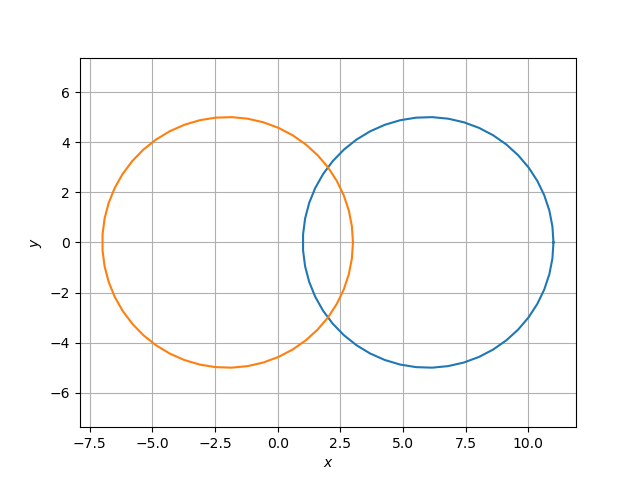
\includegraphics[width=\columnwidth]{chapters/11/11/1/12/figs/conic.png}
		\caption{}
		\label{fig:11/11/1/12}
  	\end{figure}
\iffalse
=======
Find the equation of circle passing with radius $5$ whose center lies on x-axis and passes through point $(2,3)$.
>>>>>>> f531642 (Created codes and figs folder)
\maketitle
\section{Solution:}
\begin{figure}[h]
	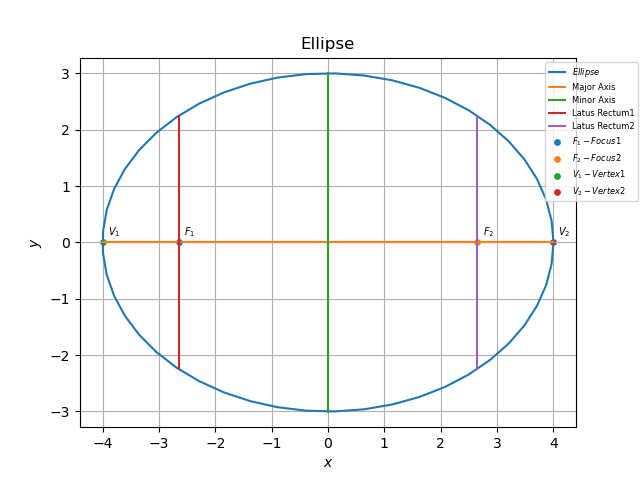
\includegraphics[width=\linewidth]{conic.png}
\caption{Circle}
\end{figure}
\subsection{Theory:}
The circle equation when it's center and radius are given is
\begin{align}
<<<<<<< HEAD
	&\vec{(x-a)^2} + \vec{(y-b)^2} = \vec{r^2}\\
\end{align}
where the centre of the circle is $\myvec{a\\b}$.
\subsection{Mathematical Calculation:}
Given the radius of circle is $5$. The circle passes through a point $\myvec{2\\3}$. Also, the center of circle is assumed as $\myvec{a\\0}$. Substitute $\myvec{a\\0}$ in eq.$1$ we get,
\begin{align}
	&\vec{(x-a)^2} + \vec{(y)^2} = \vec{25}\\
\end{align}
As the point $\myvec{2\\3}$ passes through the circle, substitute $\myvec{2\\3}$ in the equation, we get,
\begin{align}
	&\vec{(2-a)^2} + \vec{(3)^2} = \vec{25}\\
	&\vec{4+a^2-2a} + \vec{9} = \vec{25}\\
	&\vec{a^2-2a+13} = \vec{25}\\
	&\vec{a^2-2a-12} = 0\\
\end{align}
The roots of the equation will be $(6,-2)$. Hence, the center of the circle can be $\myvec{6\\0}$ or $\myvec{-2\\0}$.
The equation of circle will therefore be,
\begin{align}
	&\vec{(x-6)^2} + \vec{y^2} = 25\\
	&\vec{(x+2)^2} + \vec{y^2} = 25
=======
	&\vec{x^Tx} + \vec{2u^Tx} + c = 0\\
	&\vec{x} = \myvec{x\\y}\\\vec{u} = \myvec{g\\f}\\
\end{align}
where the centre of the circle is $\myvec{-g\\-f}$.
\subsection{Mathematical Calculation:}
Given the radius of circle is 5, the center lies on x-axis. The circle passes through a point $\vec{P} = \myvec{2\\3}$. We can get below equations,
\fi
From the given information, the following equations can be formulated
using 
	\eqref{eq:circ-eq}.
\begin{align}
		\label{eq:11/11/1/12/1}
	\norm{\vec{P}}^2 + 2 \vec{u}^{\top}\vec{P} + f &= 0
	\\
		\label{eq:11/11/1/12/2}
	\vec{u} &= k\vec{e}_1
	\\
		\label{eq:11/11/1/12/3}
	\norm{\vec{u}}^2 - f &= r^2
\end{align}
where 
\begin{align}
	\vec{P} = \myvec{2\\3} \text{ and } r = 5
\end{align}
From 
		\eqref{eq:11/11/1/12/1}
		and 
		\eqref{eq:11/11/1/12/3},
\begin{align}
	\norm{\vec{P}}^2 + 2 \vec{u}^{\top}\vec{P} + \norm{\vec{u}}^2 &= r^2
\end{align}
Substituting from 
		\eqref{eq:11/11/1/12/2} in the above, 
\begin{align}
	k^2  + 2k \vec{e}_1^{\top}\vec{P} + \norm{\vec{P}}^2- r^2 = 0
\end{align}
resulting in 
\begin{align}
	k =  - \vec{e}_1^{\top}\vec{P} \pm \sqrt{\brak{{ \vec{e}_1^{\top}\vec{P}  }}^2 + r^2 - \norm{\vec{P}}^2 } 
\end{align}
Substituting numerical values, 
\begin{align}
	k = 2, -6
\end{align}
resulting in circles with centre
\begin{align}
	-\vec{u} = \myvec{-2 \\ 0} \text{ or } \myvec{6 \\ 0}.
\end{align}
This is verified in Fig. 
		\eqref{fig:11/11/1/12}.
\iffalse
Now,
\begin{align}
	&\myvec{0*u_x\\u_y} = \myvec{0\\0}\\
	&u_y=0\\
	&13+2\myvec{u_x\\0}\myvec{2 &3}+f = 0\\
	&\myvec{u_x\\0}\myvec{u_x &0} - f = 25
\end{align}
Solving the above yield us to the points $\myvec{-2\\0}$ and $\myvec{6\\0}$.
\begin{align}
	&\vec{x^Tx} + \vec{2u^Tx} + c = 0
\end{align}
We know that $\vec{x} = \myvec{2\\3}$ and centre $\vec{u} = \myvec{-2\\0},\myvec{6\\0}$. Substitute them.
\begin{align}
	&\vec{x^Tx} + 2\myvec{-6 &0}\vec{x} + c1 = 0\\
	&\vec{x^Tx} + 2\myvec{2 &0}\vec{x} + c2 = 0
\end{align}
The value of c is $c = g^2+f^2-r^2$. Hence c can be $11,-21$. On substitution we get, the circle equations as,
\begin{align}
	&\vec{x^Tx} + \myvec{-6 &0}\vec{x} + 11 = 0\\
	&\vec{x^Tx} + \myvec{2 &0}\vec{x} + -21 = 0\\
>>>>>>> f531642 (Created codes and figs folder)
\end{align}
\section{Construction:}

\begin{table}[h]
        \centering
\setlength\extrarowheight{2pt}
        \begin{tabular}{|c|c|c|}
                \hline
                \textbf{variable} & \textbf{length/point} & \textbf{Description}\\
                \hline
		A & np.roots(coeff) & coeff = (1,-4,-12)\\
		\hline
		c & $(a-A[0])^2+b^2-r^2$ & Circle Eqn\\
		\hline
        \end{tabular}
\end{table}
\end{document}
\fi


  \item Find the equation of the circle passing through $(0,0)$ and making intercepts $a$ and $b$ on the coordinate axes.

  \item Find the equation of a circle with centre $(2,2)$ and passes through the point $(4,5)$.

  \item Does the point $(-2.5,3.5)$ lie inside, outside or on the circle $x^{2}+y^{2}=25?$
\item Find the centre of a circle passing though the points $(6,-6), (3,-7)$ and $(3,3)$. \\ 
\label{chapters/10/7/4/3}
\\
\iffalse
\documentclass[12pt]{article}
\usepackage{graphicx}
\usepackage[none]{hyphenat}
\usepackage{graphicx}
\usepackage{listings}
\usepackage[english]{babel}
\usepackage{graphicx}
\usepackage{caption} 
\usepackage{booktabs}
\usepackage{array}
\usepackage{amssymb} % for \because
\usepackage{amsmath}   % for having text in math mode
\usepackage{extarrows} % for Row operations arrows
\usepackage{listings}
\lstset{
  frame=single,
  breaklines=true
}
\usepackage{hyperref}
  
%Following 2 lines were added to remove the blank page at the beginning
\usepackage{atbegshi}% http://ctan.org/pkg/atbegshi
\AtBeginDocument{\AtBeginShipoutNext{\AtBeginShipoutDiscard}}


%New macro definitions
\newcommand{\mydet}[1]{\ensuremath{\begin{vmatrix}#1\end{vmatrix}}}
\providecommand{\brak}[1]{\ensuremath{\left(#1\right)}}
\providecommand{\norm}[1]{\left\lVert#1\right\rVert}
\providecommand{\abs}[1]{\left\vert#1\right\vert}
\newcommand{\solution}{\noindent \textbf{Solution: }}
\newcommand{\myvec}[1]{\ensuremath{\begin{pmatrix}#1\end{pmatrix}}}
\let\vec\mathbf


\begin{document}

\begin{center}
\title{\textbf{Circles}}
\date{\vspace{-5ex}} %Not to print date automatically
\maketitle
\end{center}
\setcounter{page}{1}

\section{11$^{th}$ Maths - Chapter 10}
This is Problem-3 from Exercise 10.4
\begin{enumerate}
\fi
\solution 
The equation of the circle is given by 
\begin{align}
	\label{eq:10/7/4/3circEq1}
	\norm{\vec{x}}^2+2\vec{x}^\top\vec{u}+f = 0 
\end{align}
where
\begin{align}
	\vec{u} = -\vec{c} \text{ and } \\
        \label{eq:10/7/4/3fRelation}
	f = \norm{\vec{c}}^2 - r^2
\end{align}
Given points are 
\begin{align}
	\label{eq:10/7/4/3circPoints}
     \vec{x_1} = \myvec{6 \\ -6} , \vec{x_2} = \myvec{3 \\-7}, \vec{x_3}= \myvec{3 \\ 3}
\end{align}
Substituting points from \eqref{eq:10/7/4/3circPoints} into \eqref{eq:10/7/4/3circEq1}
\begin{align}
	\brak{6^2 + \brak{-6}^2}+2\myvec{6 & -6}\vec{u}+f = 0 \\ 
	\implies 2\myvec{6 & -6}\vec{u} + f = -72 \\ 
	\brak{3^2 + \brak{-7}^2}+2\myvec{3 & -7}\vec{u}+f = 0 \\ 
	\implies 2\myvec{3 & -7}\vec{u} + f = -58 \\
	\brak{3^2 + 3^2}+2\myvec{3 & 3}\vec{u}+f = 0 \\ 
	\implies 2\myvec{3 & 3}\vec{u} + f = -18 
\end{align}
Representing the above system of equations in matrix form
\begin{align}
 \myvec{6 & -14 & 1 \\
	12 & -12 & 1 \\
	6 & 6 & 1
	} \myvec {\vec{u} \\
	           f 
		}  = \myvec{-58 \\ -72 \\ -18 }
\end{align}

The augmented matrix is expressed as
\begin{align}
	\myvec{6 & -14 & 1 & \vrule & -58 \\ 
	      12 & -12 & 1 & \vrule & -72 \\
	       6 &  6  & 1 & \vrule & -18 
	     }  
\end{align}
Performing sequence of row operations to transform into an Echelon form
\begin{align}
	\xleftrightarrow[]{{R_2\rightarrow R_2-2R_1}}  
	\myvec{6 & -14 & 1 & \vrule & -58 \\ 
	       0 &  16 & -1 & \vrule & 44 \\
	       6 &  6  & 1 & \vrule & -18 
	     }  \\ 
	\xleftrightarrow[]{{R_3\rightarrow R_3-R_1}}  
	\myvec{6 & -14 & 1 & \vrule & -58 \\ 
	       0 &  16 & -1 & \vrule & 44 \\
	       0 &  20  & 0 & \vrule & 40 
	     }  
\end{align}
\begin{align}
	\xleftrightarrow[]{{R_3\rightarrow R_3-\frac{20}{16}R_2}}  
	\myvec{6 & -14 & 1 & \vrule & -58 \\ 
	       0 &  16 & -1 & \vrule & 44 \\
	       0 &  0  &  \frac{20}{16} & \vrule & -15 
	     }  \\ 
	\xleftrightarrow[R_2\rightarrow \frac{1}{16}R_2 \text{,} R_3\rightarrow \frac{16}{20}R_3]{{R_1\rightarrow \frac{1}{6}R_1}}  
	\myvec{1 & -\frac{14}{6} & \frac{1}{6} & \vrule & -\frac{58}{6} \\ 
	       0 &  1 & -\frac{1}{16} & \vrule & \frac{44}{16} \\
	       0 &  0  &  1  & \vrule & -12 
	     }   
\end{align}
\begin{align}
	\xleftrightarrow[R_2\rightarrow R_2+\frac{1}{16}R_3]{{R_1\rightarrow R_1-\frac{1}{6}R_3}}  
	\myvec{1 & -\frac{14}{6} & 0 & \vrule & -\frac{46}{6} \\ 
	       0 &  1 & 0 & \vrule & 2 \\
	       0 &  0  &  1  & \vrule & -12 
	     }  \\ 
	\label{eq:10/7/4/3Solution}
	\xleftrightarrow[]{{R_1\rightarrow R_1+\frac{14}{6}R_2}}  
	\myvec{1 &  0 & 0 & \vrule & -3\\ 
	       0 &  1 & 0 & \vrule & 2 \\
	       0 &  0 & 1 & \vrule & -12 
	     }  
\end{align}
So, from  \eqref{eq:10/7/4/3Solution} 
\begin{align}
	\vec{u} = \myvec{-3 \\ 2} \\ 
	f = -12 
\end{align}
Since $\vec{u} = -\vec{c}$ , 
\begin{align}
	\vec{c} &= \myvec{ 3 \\ -2} \\
	\eqref{eq:10/7/4/3fRelation} \implies r^2 &= \brak{3^2 + \brak{-2}^2} + 12 \\
	 r &= 5
\end{align}
Therefore, the equation of the circle is 
\begin{align}
	\norm{\vec{x}-\myvec{3 \\ -2}}  = 5 
\end{align}
The relevant diagram is shown in Figure \ref{fig:10/7/4/3Fig1}
\begin{figure}[!h]
	\begin{center}
		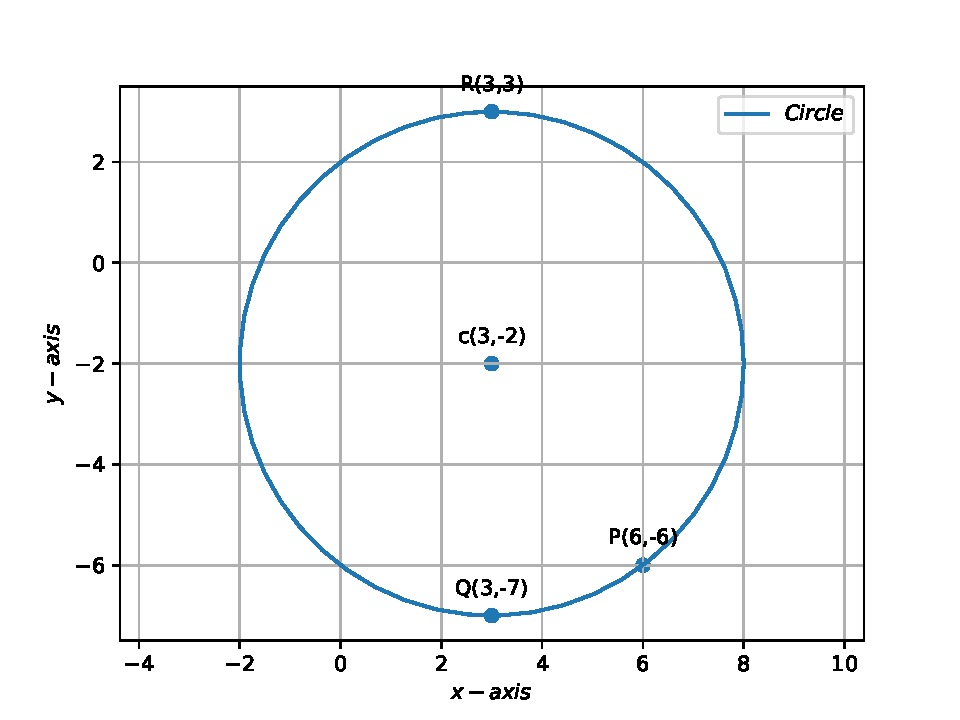
\includegraphics[width=\columnwidth]{chapters/10/7/4/3/figs/problem3.pdf}
	\end{center}
\caption{}
\label{fig:10/7/4/3Fig1}
\end{figure}

\end{enumerate}
